% Chapter 1

% useful variables
\newcommand{\plotdir}{chapters/chapter3/plots}

\chapter{Data analysis} % Main chapter title
\label{chapter3} % For referencing the chapter elsewhere, use \ref{Chapter1} 

% ----------------------------------------------------------------------------------------

\section{General Analysis approach}
\label{chapter3:sec:analysis-approach}

\section{Geant4 simulation of the experiment}
\label{chapter3:sec:geant4}

\subsection{Correction of longitudinal shower profile in the Hadronic calorimeter}
\label{chapter3:sec:geant4-hcal-corr}

\subsection{Output digitization}
\label{chapter3:sec:geant4-digitization}

\subsection{Signal simulation}
\label{chapter3:sec:geant4-signal}

\section{Background}
\label{chapter3:sec:bkg}

\subsection{Heavy charged particle rejection using synchrotron radiation}
\label{chapter3:sec:bkg-srd}

Simulation of the expected SR signal was performed with the Geant 4 package\cite{ALLISON2016186,1610988,AGOSTINELLI2003250}.
The geometry of the NA64 experiment was coded in Geant 4, including the 200 $\mu$m mylar vacuum windows, the detailed composition of the trackers, scintillators and the residual gas was set at a level of $10^{-3}$ mBar as in the measurements. Saturation of BGO was taken into account using Birks' law with the constants taken from \cite{AVDEICHIKOV2002251}.

The expected SR spectra for pions and electrons with energies of 50 GeV and 100 GeV are shown in Fig. \ref{SRspectrum}. The plot shows the expected dependence on the incoming electron energy in the emission spectra for the realistic experimental conditions.
Moreover, the comparison between the SR spectra of pions and electrons illustrates clearly the principle of this technique that allows to discriminate between them by requiring an energy threshold in the synchrotron detector. 
For pions, one can see that the probability of detecting an event with energy above 1 MeV (the threshold in our detector) is about $\sim 10^{-3}-10^{-4}$.
These SR-like signals originate from the interactions of the incoming pions with material which they ionise as predicted by Eq. \ref{eqn:knock-on}.
 \par 
Furthermore, Geant 4 reproduces the critical energy $E_c$ which divides the spectrum into two parts of equal power is:
\begin{equation}
E_c = \frac{3 \hbar c \gamma^3}{2R}
\end{equation}
with the reduced Plank constant $\hbar$ and the bending radius $R$. 
 For 100 GeV electrons in the  $B=1.7$ T bending field this corresponds to $E_c\sim$11.35 MeV. The expected mean energy of a synchrotron photon $E_m=E_c/\pi\simeq 3.6$ MeV is in very good agreement with simulation. The number of photons emitted per revolution in this energy range in the field of 7 T$\cdot$m is defined as:
\begin{equation}
N_\gamma = \frac{5 \pi \alpha}{\sqrt{3}}\gamma
\end{equation}
where $\alpha$ is the fine structure constant. 
By scaling this equation for the fraction of the circle where the particles are inside the magnetic field, one obtains a mean number of emitted photon of about 24.
The SRD geometrical acceptance is about one third,  thus one can estimate that the sum of deposited energy is approximately 29.35 MeV in good agreement with the results of the simulation as shown in Fig. \ref{SRspectrum}. 
 
\begin{figure}[htb!]
\centering
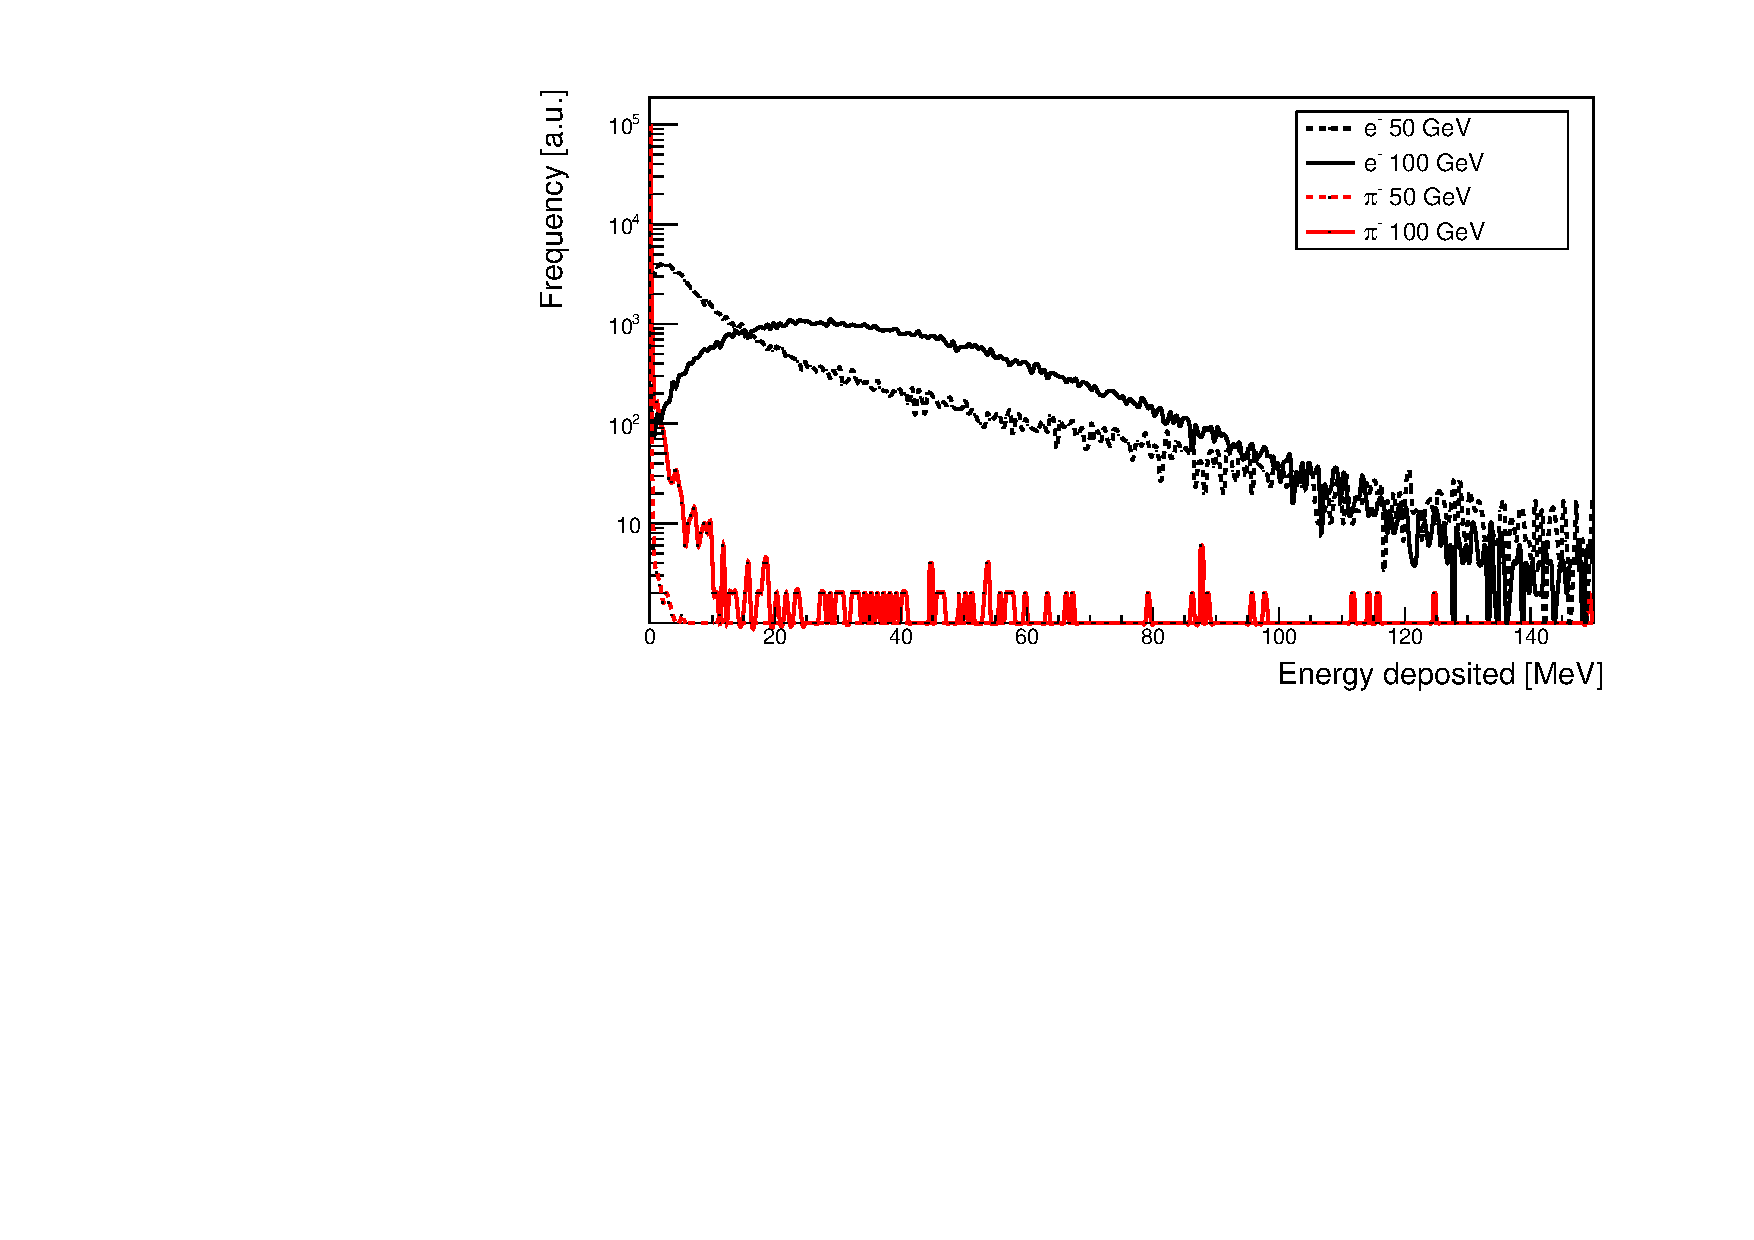
\includegraphics[width=1.\textwidth]{\plotdir/comp_spectra.pdf}
\caption{Result of the Geant 4 simulation for the energy detected by the SR detector for 50/100 GeV e$^-$(black dashed/solid line) and 50/100 GeV $\pi^-$ (red dashed/solid line).}
\label{SRspectrum}
\end{figure}

The SRD detector was tested during the NA64 test beam run in July 2016. The two BGO rows are parallel to the primary beam direction as shown in Fig.\ref{fig:newgeo}. The dipole magnets installed in series (see Fig. \ref{fig:NA64Setup}) produce a total integrated magnetic field of 7 T$\cdot$m \cite{Banerjee:2016tad} resulting in a nominal displacement for the incoming electrons at the SRD/ECAL positions of 31/34 cm from the undeflected beam axis. The SRD was placed between the undeflected and the deflected beam axis at a distance of approximately 9 cm from both (Fig.\ref{fig:newgeo}). This separation minimises the possibility for Bremsstrahlung photons and neutral particles produced by interactions of the beam particle with materials upstream (vacuum windows, collimators, trackers...) and for particles in the beam halo (most of the beam used in the experiment was constrained in a circular region with diameter 2 cm) to hit the SRD. In fact, such interactions result in the saturation of the SRD with a significant loss of efficiency due to the long decay time of the BGOs.

%The expected Landau distribution of energy deposits was fit to the data to find the mean peak position to extract the calibration constant. 

The two crystals facing the beam (labeled 3 and 7 in Fig. \ref{fig:newgeo}) detect most of the energy emitted by synchrotron radiation. We will refer to those as SRD BGOs from now on. The remaining six crystals are used to detect events with high energy deposition in the SRD. In particular the last two crystals of each row (labeled 0 and 4 in Fig. \ref{fig:newgeo}) detect some energy only in the case of very energetic Bremsstrahlung events and thus can be used as a veto (see Fig.\ref{fig:newgeo}). The six crystals after the SRD BGOs act also as a shield from backscattering particles coming from the ECAL suppressing pions by an additional order of magnitude. Finally in this geometry it is possible to use the coincidence of the two SRD BGO crystals to improve the tagging of synchrotron photons by rejecting knock-on electrons produced by incoming pions. In fact synchrotron radiation has a homogenous spectrum in the whole arc described by the primary and deflected beam and thus a signal is detected in both SRD BGOs. On the contrary, electrons generated by a $\pi^-$ undergoing ionisation will mostly leave energy only in a single crystal as illustrated in Fig. \ref{fig:newgeo}. 
With the requirement of detecting in both SRD BGOs an energy deposition above a 1 MeV the suppression factor is improved up to a level of $10^{-5}$.



\begin{figure}[htb!]
  \centering
  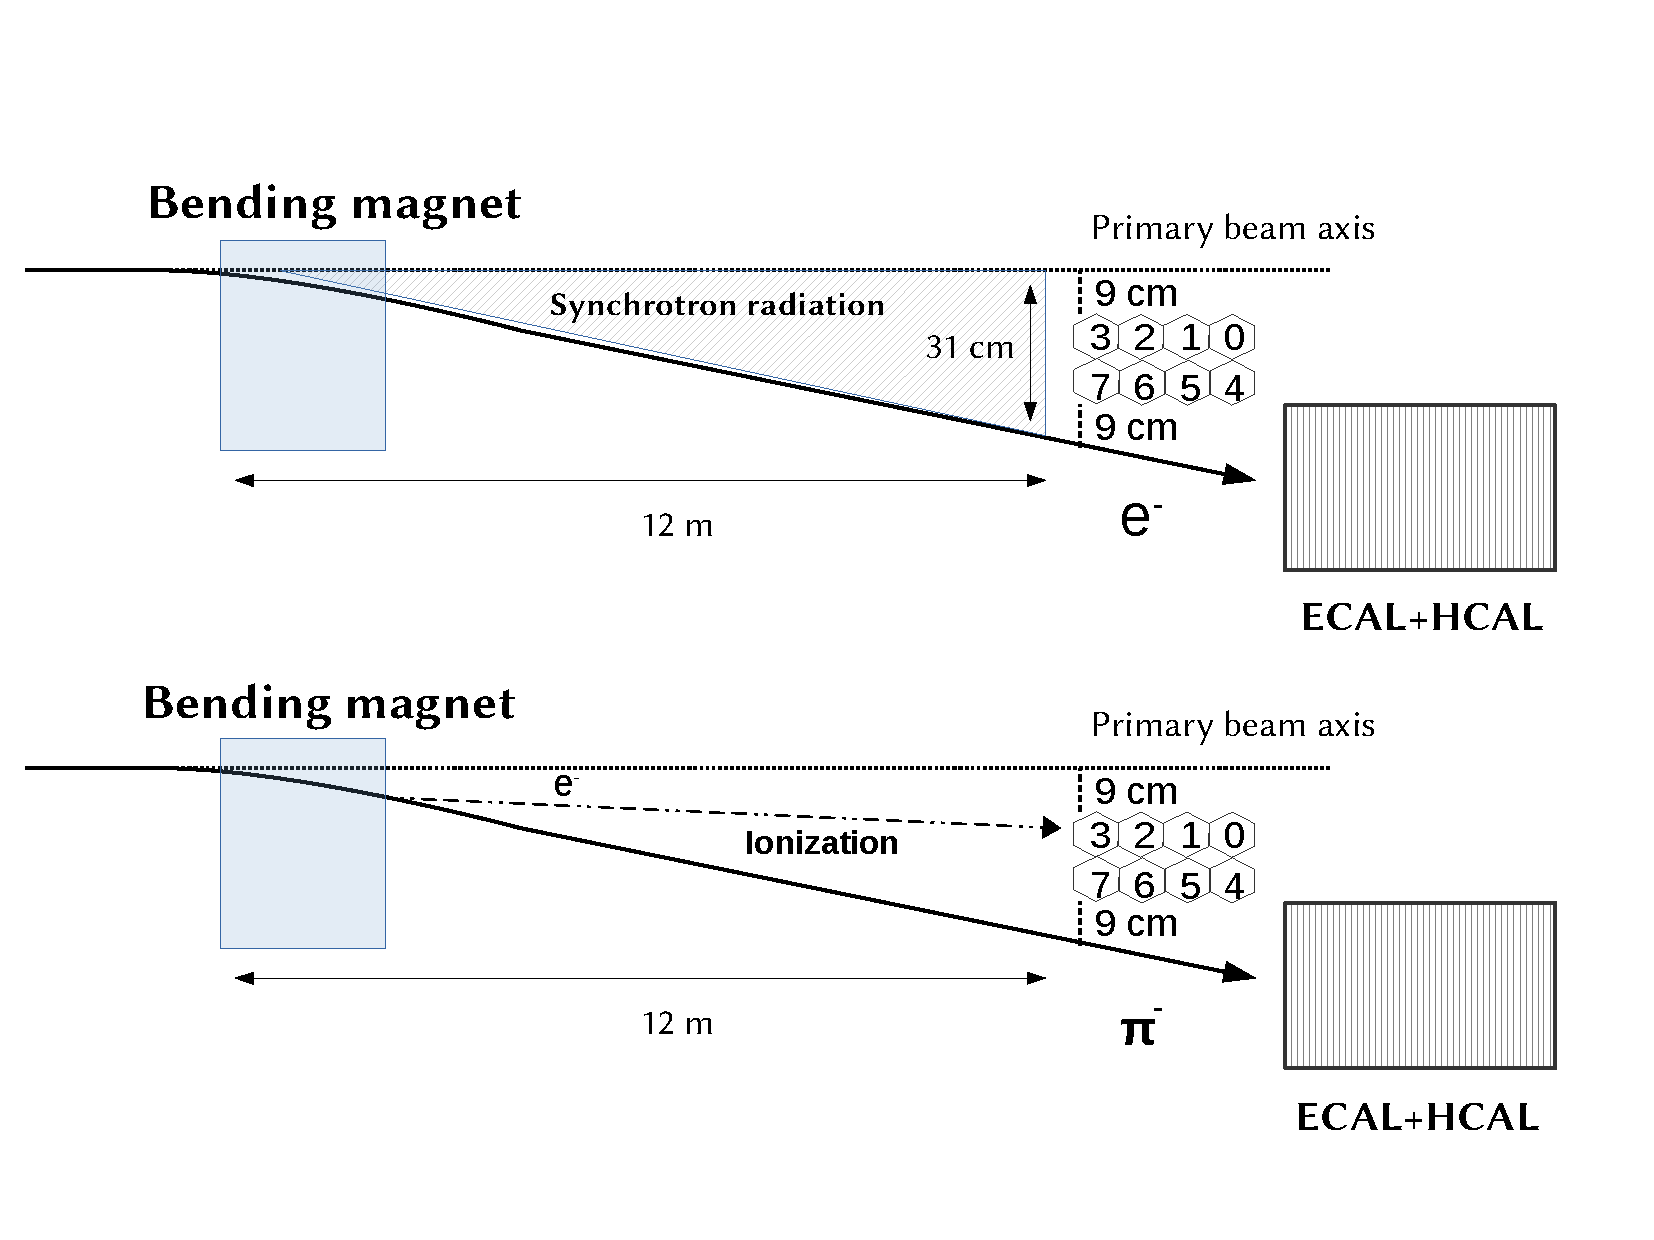
\includegraphics[width=.9\textwidth]{\plotdir/sketch.pdf}
  \caption{Geometry of the BGO crystals. Crystals 7,3 (SRD BGO) collect most of the synchrotron radiation spectrum. Crystals 4,0 (VETO BGO) on the other hand are effected only in case of a high energy event and are thus used as a veto. The remaining crystals serve as a shield for the SRD from backscattering particles coming from the ECAL. Top: illustration of event leaving a SR signal in the SRD. Bottom: illustration of a SR- like signal in the SRD for a knock-on electron produced by pions.}
\label{fig:newgeo}
\end{figure}

Data with a 100 GeV $\pi^-$ beam were taken to have a direct measurement of the suppression factor achievable through synchrotron radiation measurements. The beam intensity was 5.3$\times 10^4$ particles per spill. The trigger was given by the coincidence of the three plastic scintillator counters (S1, S2 and S3 shown in Fig.\ref{fig:NA64Setup}). The additional requirement of an energy deposition below 60 GeV in the ECAL was applied in order to select an almost pure $\pi^-$ sample of $\sim 10^5$ collected events. The probability for electrons to punch through the 40 radiation lengths of the ECAL was estimated to be at a level of $10^{-12}$ \cite{Banerjee:2016tad}. 

For the 100 GeV electron beam run, a total of 220 spills were recorded with an intensity of 3.4$\times 10^5$/spill. 
The same trigger used in the pion run was used for the electron data.
In this case though, in order to reduce the pion contamination which is at a level of few \% and obtain a pure sample of electrons-only events with a total energy deposition in ECAL + HCAL above 90 GeV but with less than 20 GeV energy in the HCAL were used.  


The energy spectra recorded by the SRD BGO with electrons and pions are shown in Fig.\ref{fig:comp_spectra}. The SR spectra obtained with the electron beam are used to perform the BGO calibration by comparison with the simulation. With this method a very good agreement of data and MC is achieved (see plot on the left of Fig.\ref{fig:comp_spectra}). As a cross check, using the obtained calibration constants, the data from the pion beam impinging directly on the SRD are fitted with a Landau distribution. The obtained peak position of 60 MeV is in good agreement with the prediction of the MC. 

Time coincidence of signals above the energy threshold of 1 MeV from both SRD counters is required and high energy Bremsstrahlung events are removed using the veto BGO.
The suppression of synchrotron radiation emission detected for pions compared to electrons is clearly visible by comparing the two plots. For the electron spectrum, a 1\% pileup beam events have been added to the simulation as predicted for the given spill intensity and with the known decay time of BGOs.  Both spectra are in very good agreement with the simulation.

\begin{figure}[htb!]
  \centering
  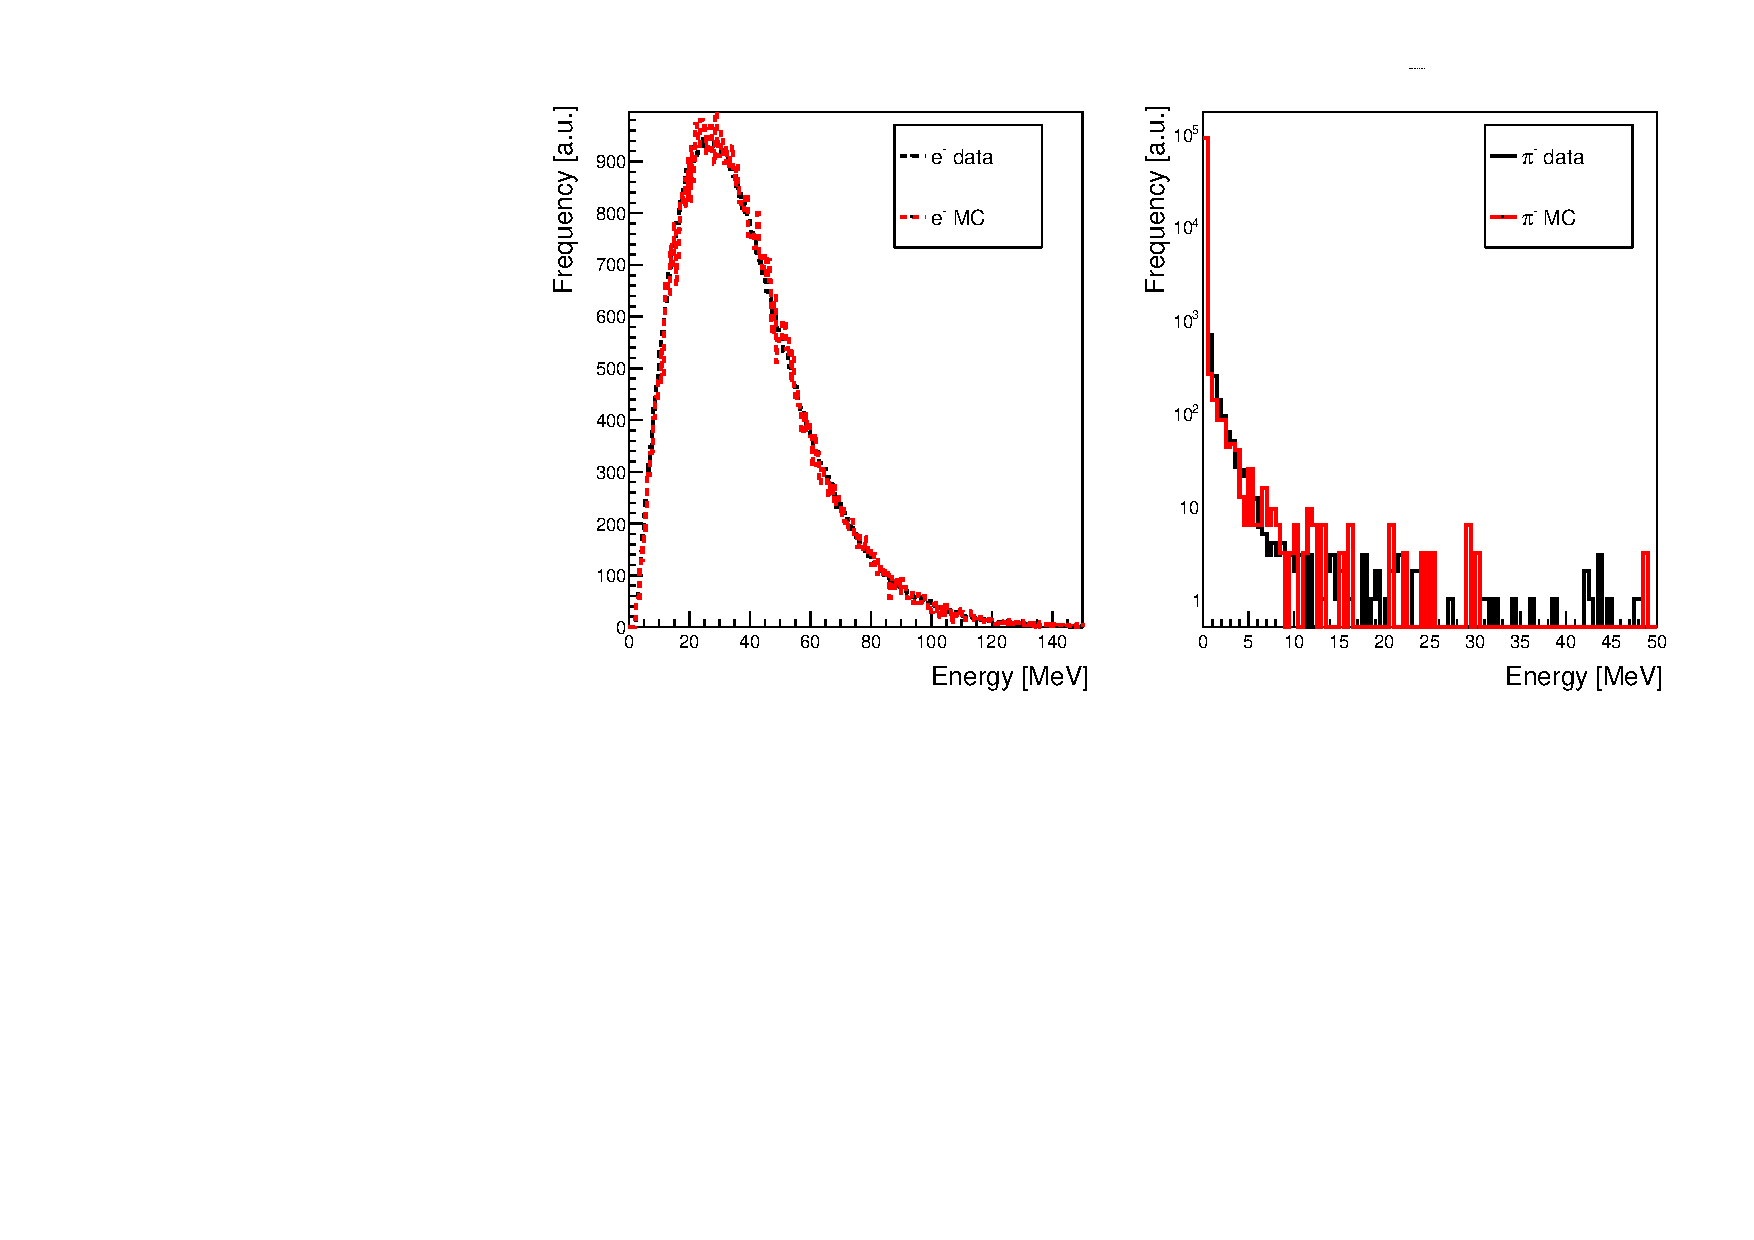
\includegraphics[width=1.\textwidth]{\plotdir/spectra_tot.pdf}
  \caption{Comparison between data and simulation (MC) of the synchrotron radiation spectrum detected for 100 GeV electrons (left) and pions (right). }
  \label{fig:comp_spectra}
\end{figure} 

\begin{figure}[htb!]
  \centering
  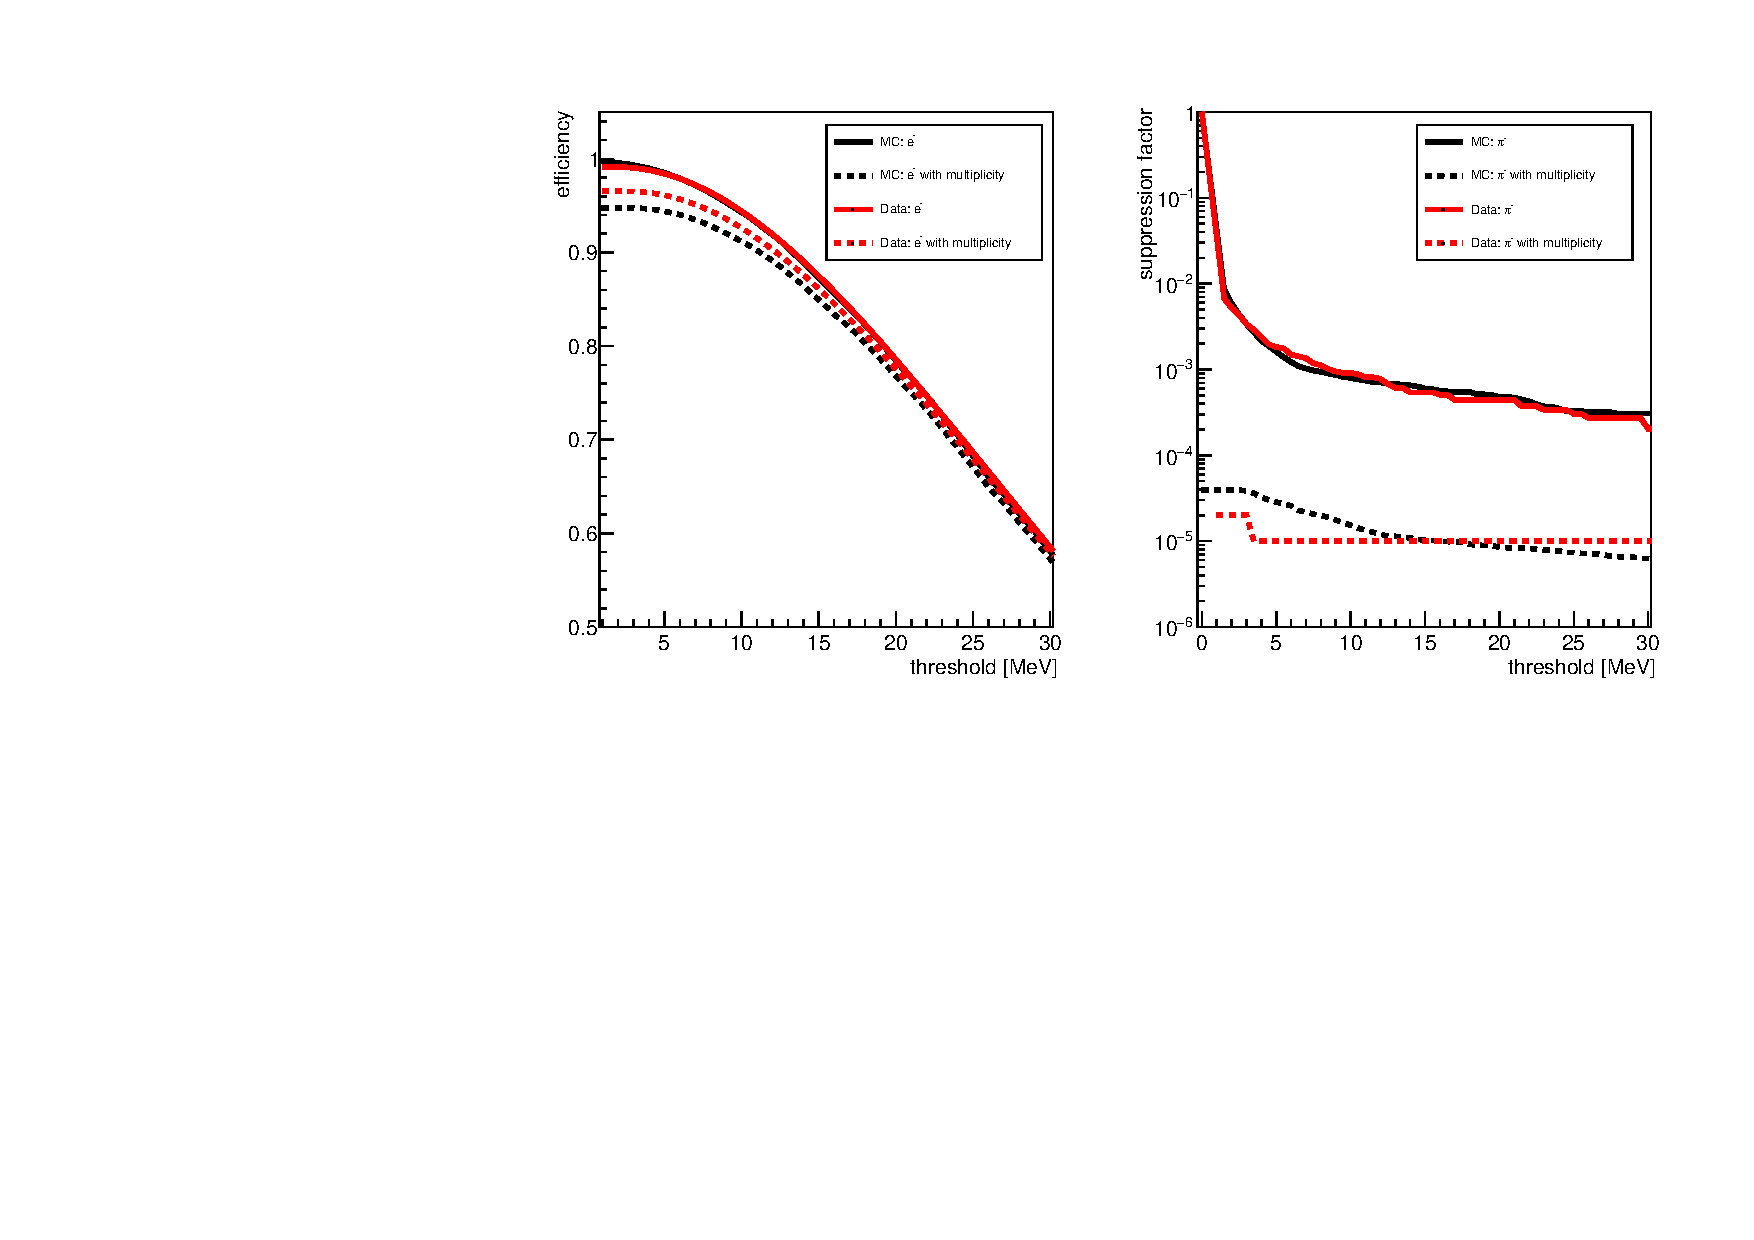
\includegraphics[width=1.\textwidth]{\plotdir/sup_mult.pdf}
  \caption{Left: Comparison between data and simulation (MC) for electrons of the efficiency as a function of threshold set on the total energy deposited in the SRD BGO and for the requirement that this is deposited in each single crystal (multiplicity). Right: Comparison between data and simulation for pions and electrons of the suppression factor as a function of the threshold set on the total energy deposited in the SRD BGO and for the multiplicity requirement.}
  \label{fig:sup_mult}
\end{figure}

The efficiency for the electrons and the suppression factor for the pions are plotted in Fig. \ref{fig:sup_mult} as a function of the threshold on the energy deposited in the SRD. We distinguish between two cases:
\begin{enumerate}
\item The threshold is set on the total energy deposited in the SRD.
\item Both SRD signals have to be in-time and above the threshold of 1 MeV (multiplicity requirement).
\end{enumerate}
One can see that applying the criterion 2) the efficiency only decreases slightly compared to 1), while the suppression factor for pions is dramatically increased (by two orders of magnitude) with the requirement of having the two BGOs in coincidence.
This can be understood because the SR-like signal generated from secondary electron will leave a signal only in one of the two BGOs while the SR from electrons is spread out uniformly as explained above. 
This is also nicely evidenced by Tab. \ref{tab:hits} where the fraction of events with different hit multiplicity in the SRD BGO for both pion and electron runs are reported.

\begin{table}[hbt!]
\begin{center}
\begin{tabular}{cccc}
Events hit multiplicity  (\%) & 0 BGO  & 1 BGO & 2 BGOs\\
\hline
Pions & $98.77$ & $1.21$ & $1.4\times10^{-3}$  \\
Electrons & $2.4\times10^{-1}$  & $2.60$ & $97.37$ \\
\end{tabular}
\end{center}
\caption{Fraction of pion and electron events for different hit multiplicity in the SRD from the data.}
\label{tab:hits}

\end{table}

\subsection{Hadron rejection using electromagnetic shower profile}
\label{chapter3:sec:bkg-ecal-profile}

\subsection{Study of K$^0_S$ background in visible mode}
\label{chapter3:sec:bkg-k0s}

\subsection{Study of neutral punch-through in the Calorimeters}
\label{chapter3:sec:bkg-neutrals}

\section{Study of $\gamma + Z \rightarrow \mu^+ \mu^-$ events }
\label{chapter3:sec:dimuons}


\subsection{Vertex and angle reconstruction}
\label{chapter3:sec:dimuons-reco}

\subsection{Signal yield correction}
\label{chapter3:sec:dimuons-sig-corr}

\section{Selection criteria}
\label{chapter3:sec:selection-criteria}

\subsection{Invisible mode}
\label{chapter3:sec:selection-criteria-invis}

\subsection{Visible mode}
\label{chapter3:sec:selection-criteria-vis}

\subsubsection{Analysis using Veto at the end of the dump}
\label{chapter3:sec:vis-mode-veto}

\subsubsection{Mixed approach using tracking and Veto}
\label{chapter3:sec:vis-mode-tracking}

%%% Local Variables:
%%% mode: latex
%%% TeX-master: t
%%% End:
